\chapter{Correlation and Linear Regression}
\section{Scatter Diagrams}
\begin{note}
  Guidelines for drawing a scatter diagram
  \begin{itemize}
    \item The relative position of each point on the scatter diagram should be clearly shown.
    \item The range of values for the set of data should be clearly shown by marking out the extreme \(x\) and \(y\) values on the corresponding axis.
    \item The axes should be labeled clearly with the variables.
  \end{itemize}
  \begin{figure}[H]
    \centering
    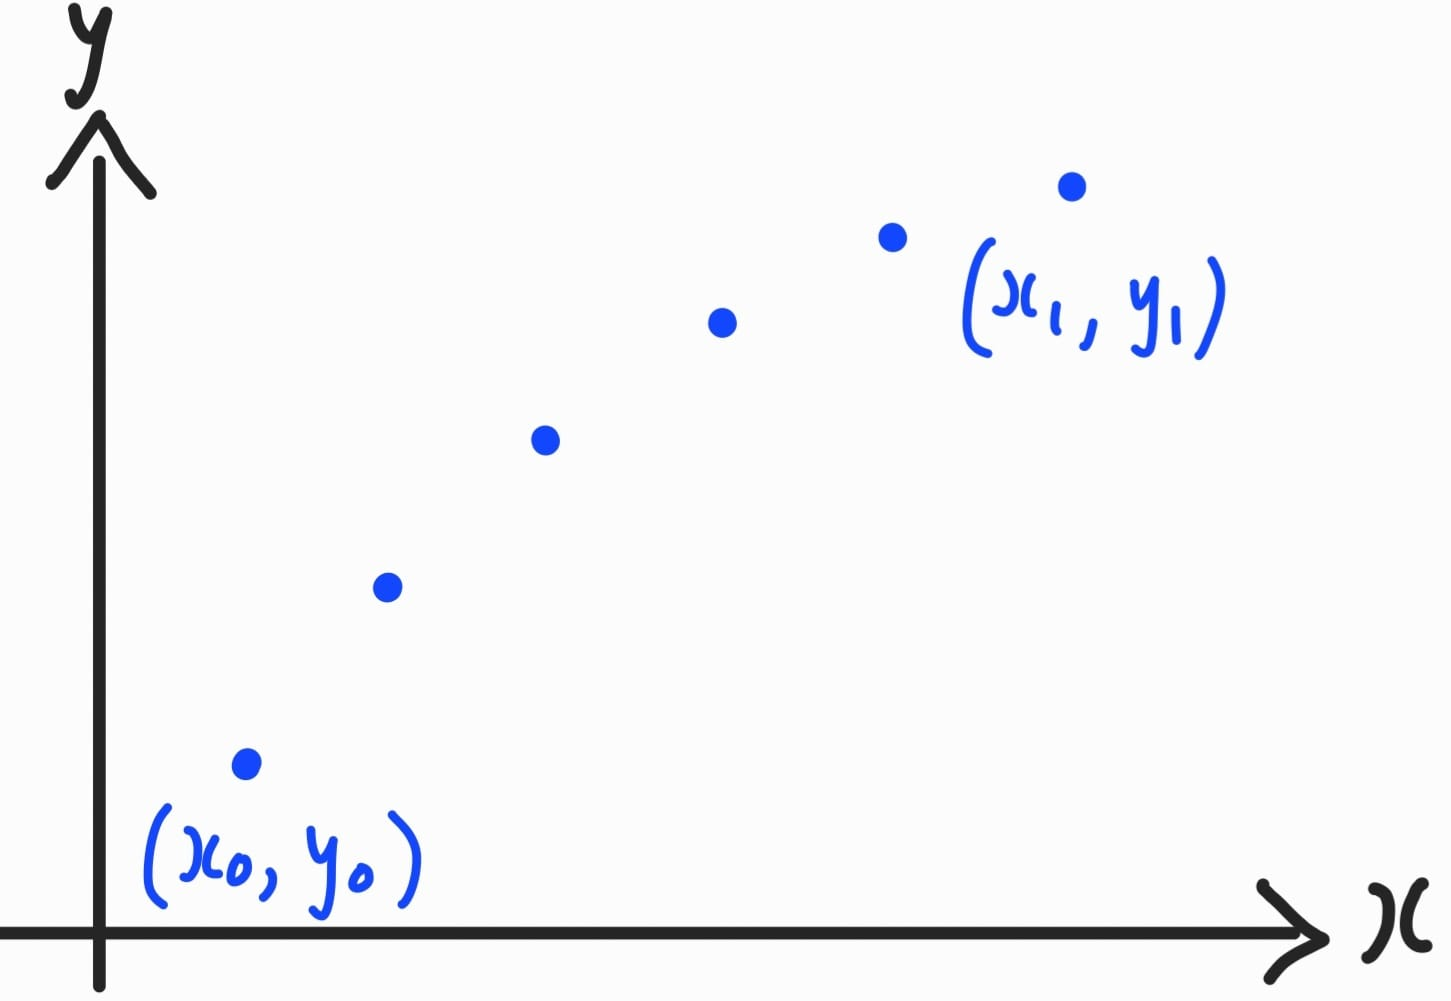
\includegraphics[width=0.4\textwidth]{../images/scatter-plot-example.jpg}
    \caption{\ref{Me} An illustration of a scatter plot.}
    \label{fig:example-scatter-plot-how-to-draw}
  \end{figure}
  \emph{Note.} We do not need to start from the origin.
\end{note}
\begin{GCSkills}{}
  To show a scatter plot on the G.C.:
  \begin{center}
    \texttt{2nd} \(\Longrightarrow\) \texttt{y=} \(\Longrightarrow\)  \texttt{1:Plot1\dots on} \(\Longrightarrow\) \texttt{enter} \(\Longrightarrow\)  \texttt{on}.
  \end{center} 
  \emph{Note.} When we no longer need a scatter plot, turn the scatter plot(s) \emph{off} in the G.C., lest it erroneously interferes with other functionalities of the G.C.
\end{GCSkills}
\begin{example}{}{}
  % N2008/II/8(iii)
  One of the values of \(t\) appears to be incorrect. Indicate the corresponding point on your diagram by labelling it \(P\) and explain why the scatter diagram for the remaining points may be consistent with a model of the form \(y=a+bf(x)\). 
  \begin{center}
    \parbox{0.9\textwidth}{
      With \(P\) removed, the remaning points seem to lie, on a curve that [e.g. increases at a decreasing rate], suggesting consistency with the model \(y=a+bf(x)\).
    }
  \end{center}
\end{example}
\section{Product Moment Correlation Coefficient \(r\)}
\begin{definition}{}{}
  The Product Moment Correlation Coefficient is a measure of the linear correlation between two variables. It is defined by
    \[r\coloneq\frac{\sum{(x-\widebar{x})(y-\widebar{y})}}{\sqrt{\sum{(x-\widebar{x})^2}\sum{(y-\widebar{y})^2}}}=\frac{\sum{xy}-\dfrac{\sum{x}\sum{y}}{n}}{\sqrt{\left[\sum{x^2}-\dfrac{\left(\sum{x}\right)^2}{n}\right]\left[\sum{y^2}-\dfrac{\left(\sum{y}\right)^2}{n}\right]}},\]
    and takes on a value from 0 to 1. See Figure \ref{fig:scatter-plot-r-value-examples} for some scatter plots of various \(r\) values.
    % \item When \(r=0\), there is no linear relationship. But, a nonlinear relationship may be present. Additionally, the regression lines are perpendicular.
    % \item The closer the value of \(r\) is to 1 (or \(-1\)), the stronger the positive (or negative) linear correlation. Furthermore, the regression lines coincide when \(\lvert r \rvert=1\).
\end{definition}
\begin{figure}[htbp]
  \centering
  \begin{subfigure}[c]{0.4\textwidth}
    \centering
    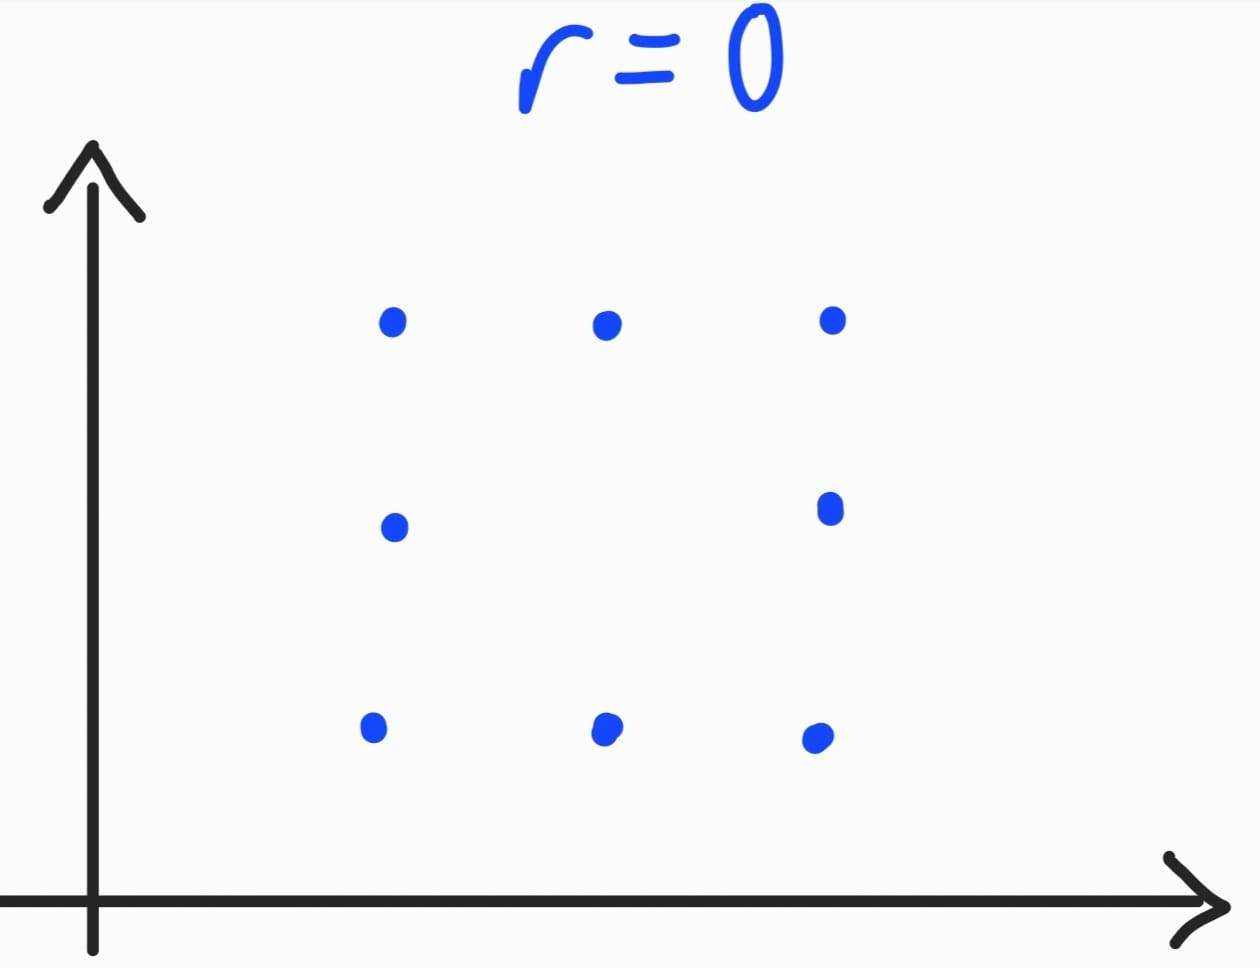
\includegraphics[width=\textwidth]{../images/product-moment-correlation-coefficient/r-is-0.jpg}
    \caption{No \emph{linear} relationship.}
  \end{subfigure}

  \begin{subfigure}[c]{0.4\textwidth}
      \centering
      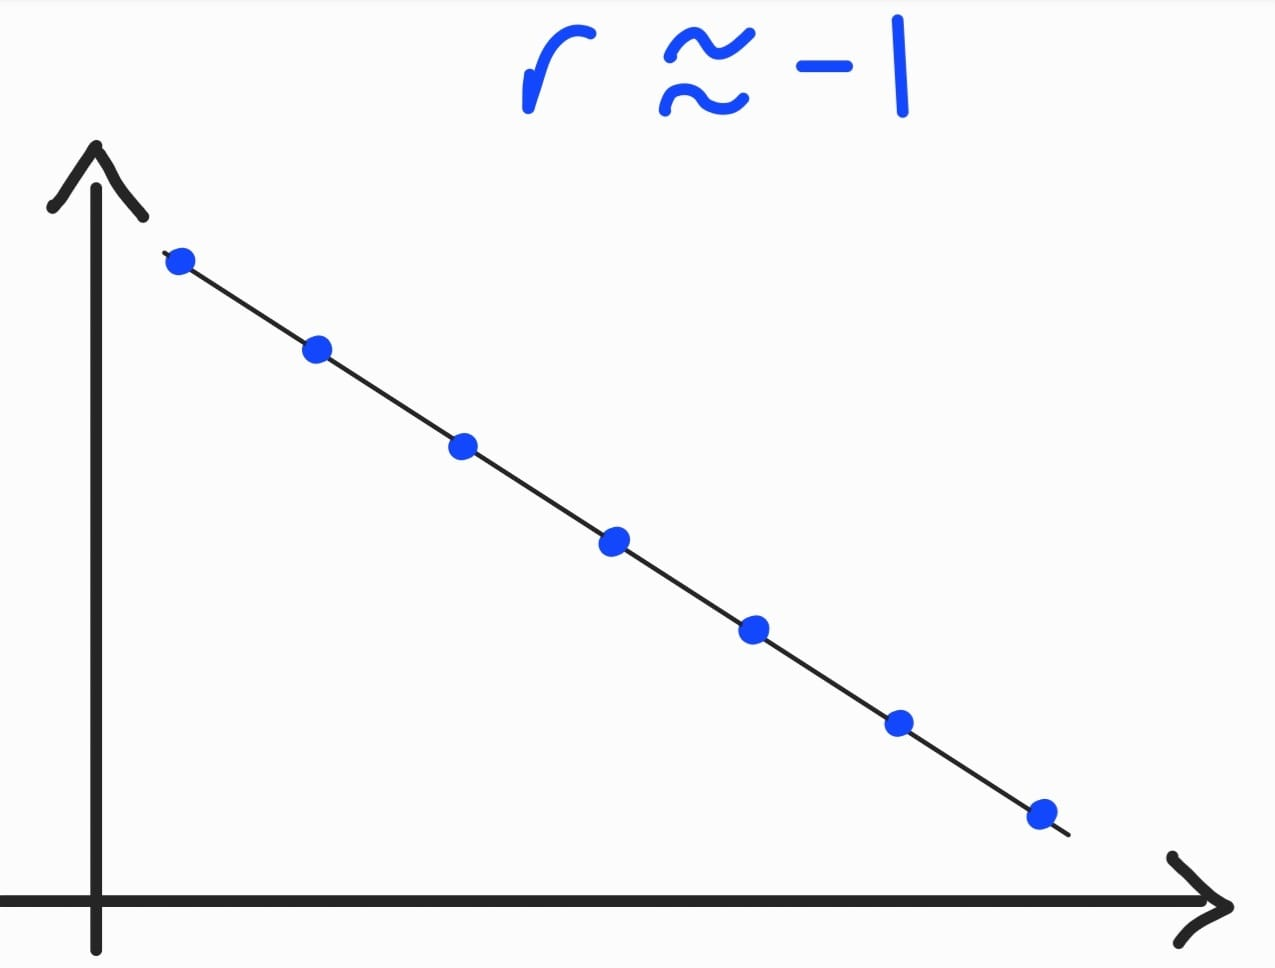
\includegraphics[width=\textwidth]{../images/product-moment-correlation-coefficient/r-is--neg-1.jpg}
      \caption{Strong negative linear relationship.}
  \end{subfigure}\hspace{0.06666666666667\textwidth}
  \begin{subfigure}[c]{0.4\textwidth}
      \centering
      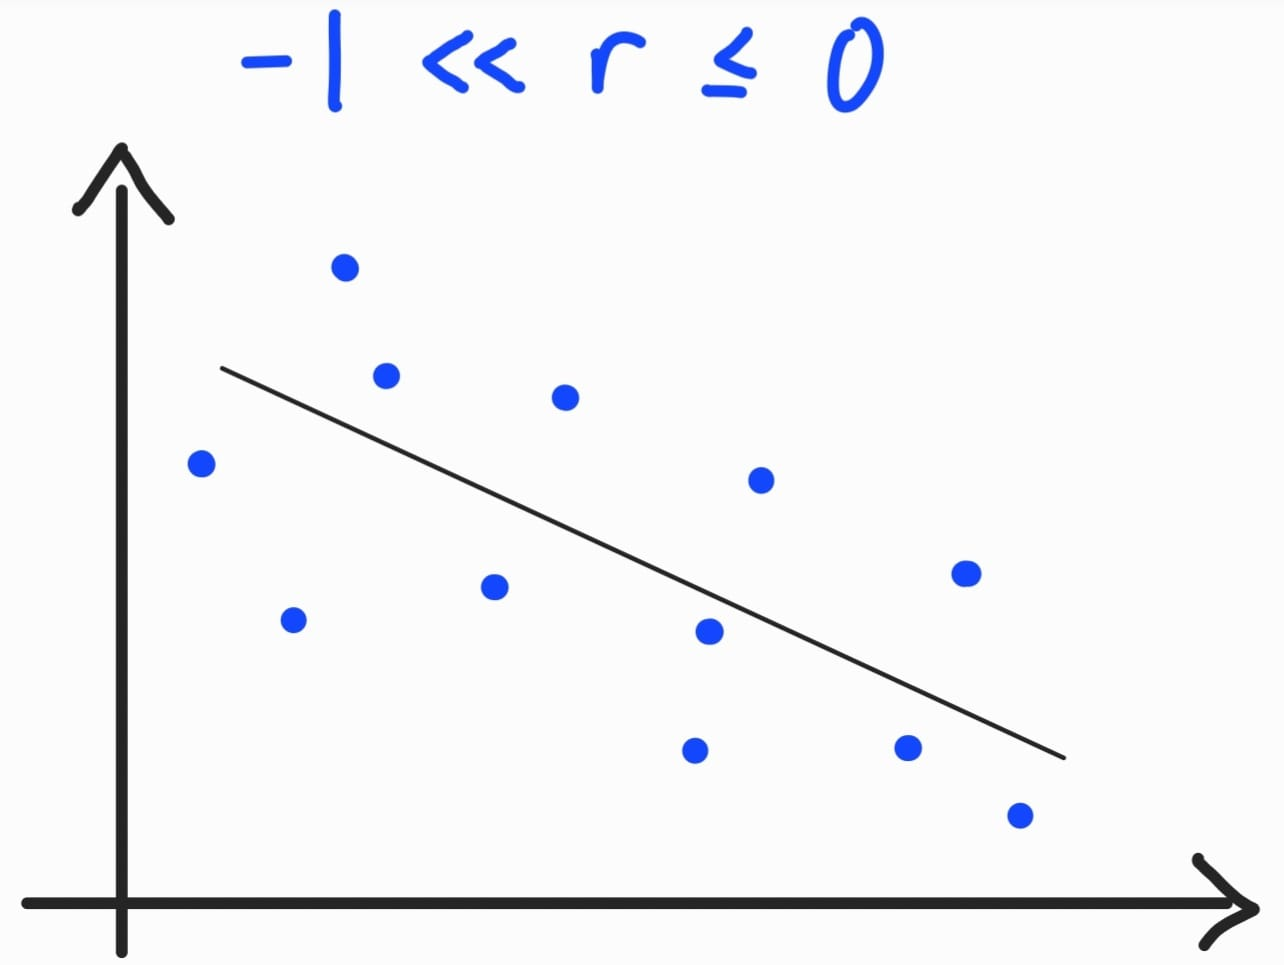
\includegraphics[width=\textwidth]{../images/product-moment-correlation-coefficient/small-negative-r.jpg}
      \caption{Weak negative linear relationship.}
  \end{subfigure}

  \begin{subfigure}[c]{0.4\textwidth}
      \centering
      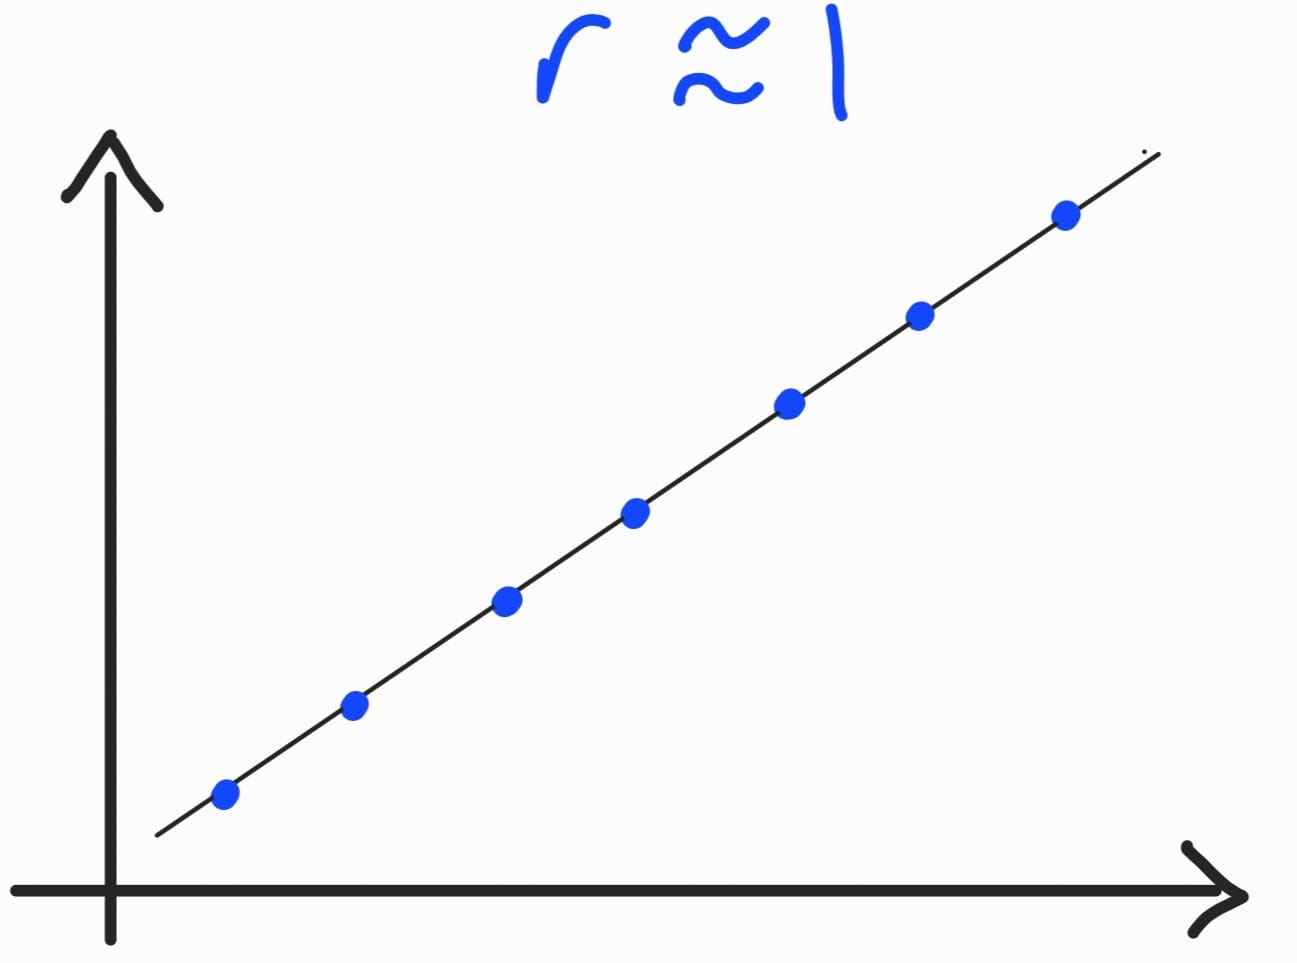
\includegraphics[width=\textwidth]{../images/product-moment-correlation-coefficient/r-is-1.jpg}
      \caption{Strong positive linear relationship.}
  \end{subfigure}\hspace{0.06666666666667\textwidth}
  \begin{subfigure}[c]{0.4\textwidth}
      \centering
      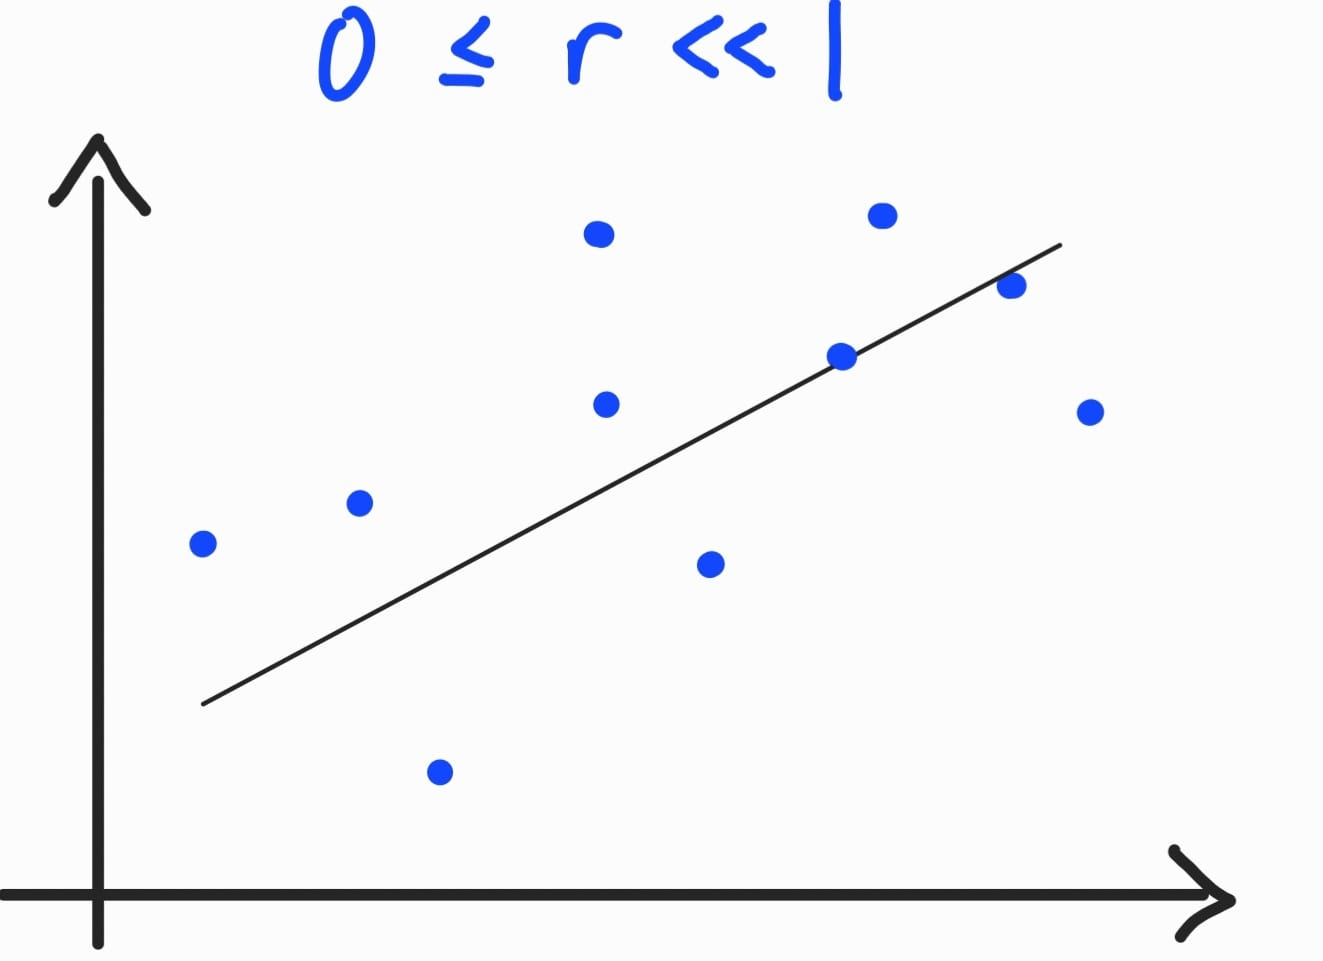
\includegraphics[width=\textwidth]{../images/product-moment-correlation-coefficient/small-positive-r.jpg}
      \caption{Weak positive linear relationship.}
  \end{subfigure}

  \begin{subfigure}[c]{0.4\textwidth}
    \centering
    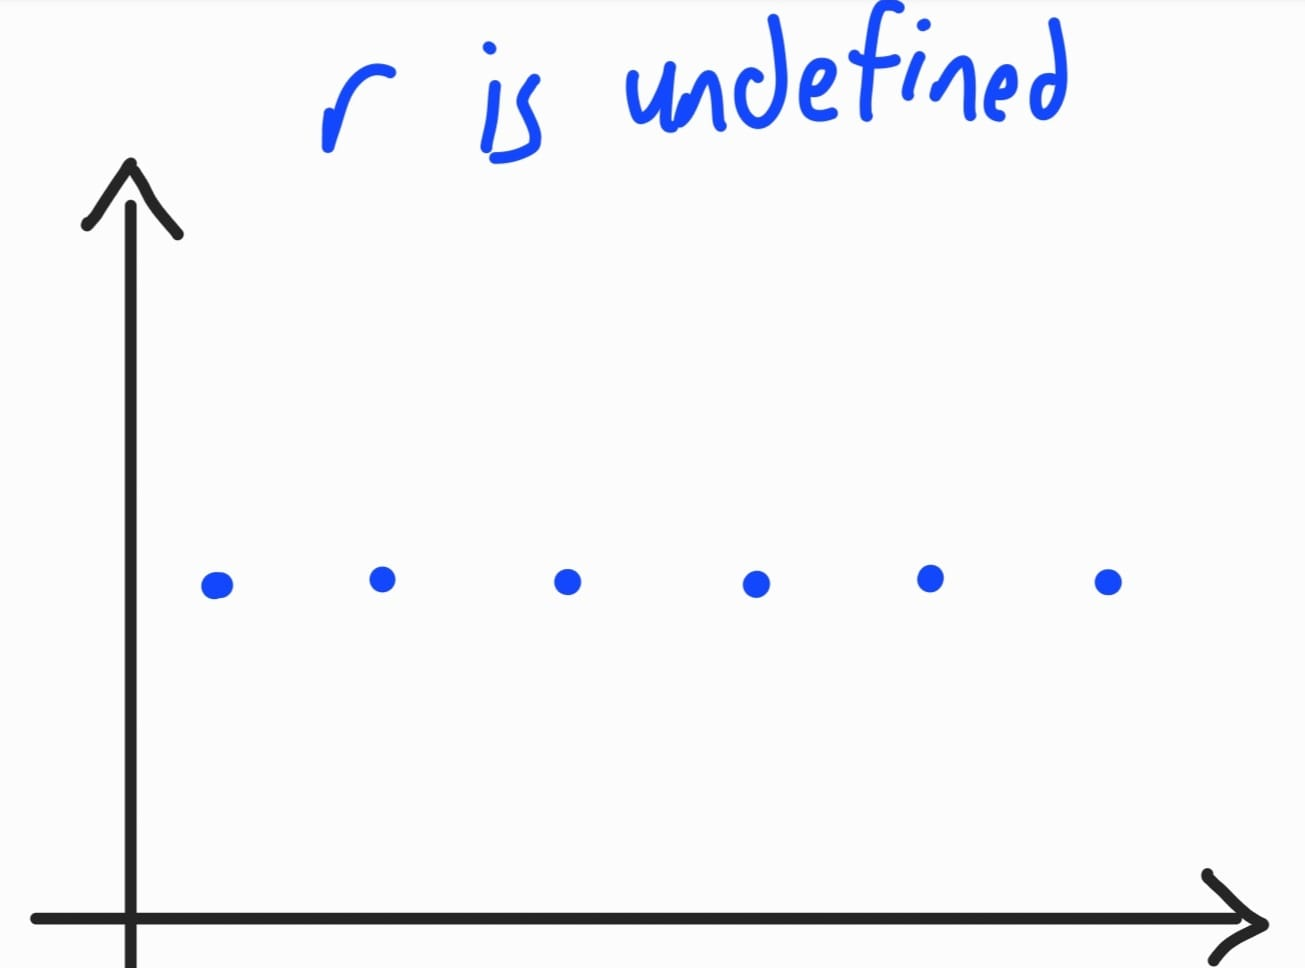
\includegraphics[width=\textwidth]{../images/product-moment-correlation-coefficient/r-is-undefined-horizontal-points.jpg}
    \caption{\(\sum{(y-\widebar{y})^2}=0\).}
  \end{subfigure}\hspace{0.06666666666667\textwidth}
  \begin{subfigure}[c]{0.4\textwidth}
    \centering
    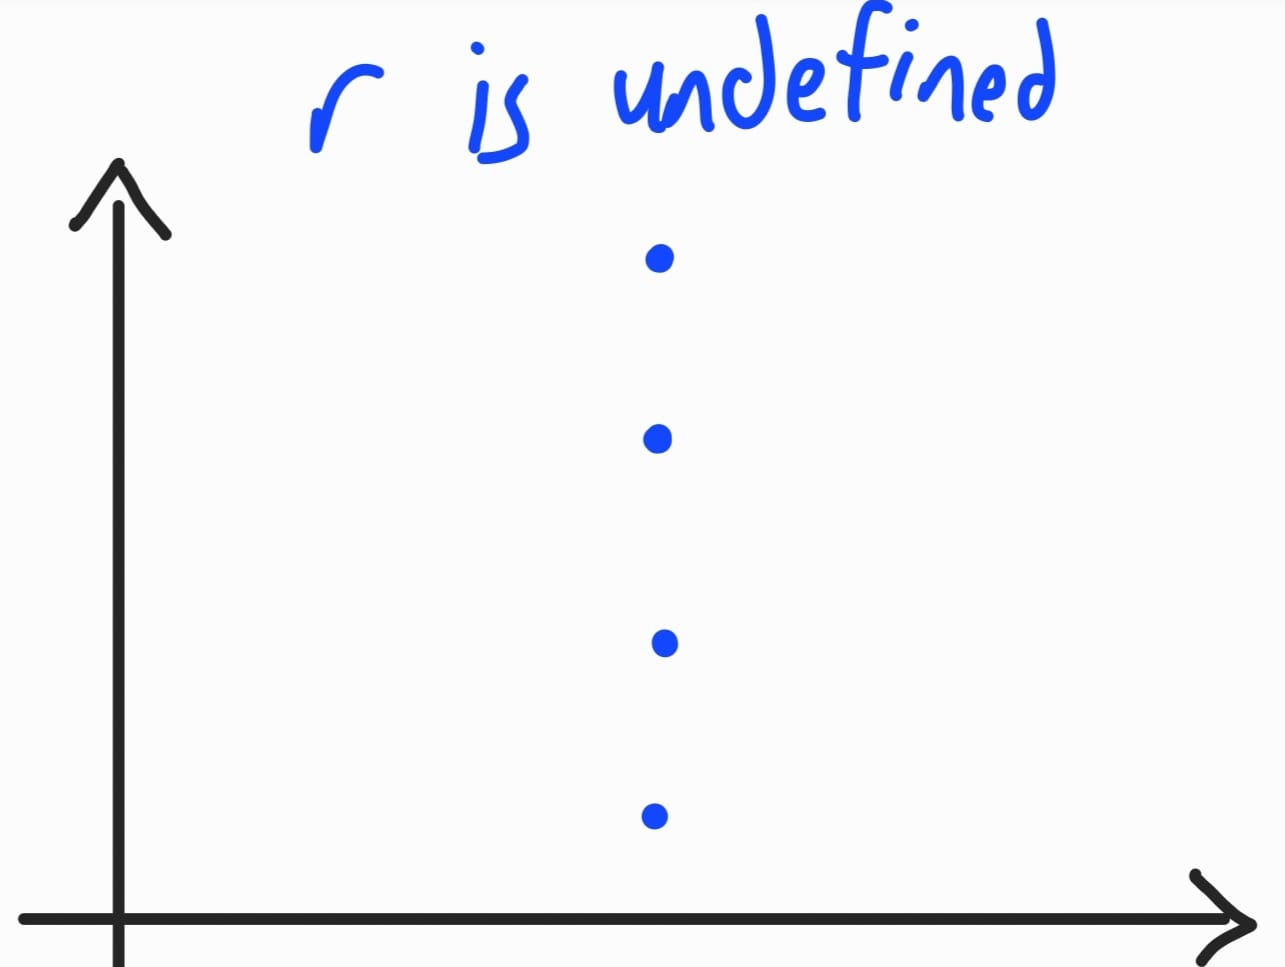
\includegraphics[width=\textwidth]{../images/product-moment-correlation-coefficient/r-is-undefined-vertical-points.jpg}
    \caption{\(\sum{(x-\widebar{x})^2}=0\).}
  \end{subfigure}
  \caption{\ref{Me} Example scatter plots with different values of \(r\).}
  \label{fig:scatter-plot-r-value-examples}
  \begin{flushleft}
    \emph{Note.} Even though there is no \emph{linear} relationship when \(r=0\), there might be a \emph{nonlinear} relationship present. 
  \end{flushleft}
\end{figure}
\begin{note}
  Explain whether your estimate using the regression line of \(y\) on \(x\) is reliable.
  \begin{center}
    \parbox{0.9\textwidth}{
      Since the \(\lvert r \rvert\) value of \rule{0.5cm}{0.01mm} is close to 1, \emph{and} \(x=\rule{0.5cm}{0.01mm}\) is within the data range of \(\rule{0.5cm}{0.01mm}\leq x\leq \rule{0.5cm}{0.01mm}\), the estimate is reliable.
    }
  \end{center}
\end{note}
\begin{note}
  Explain why the estimate using the regression line \(y\) on \(x\) is not reliable.
  \begin{center}
    \parbox{0.9\textwidth}{
      Since \(x=\rule{0.5cm}{0.01mm}\) falls outside of the range of data \(\rule{0.5cm}{0.01mm}\leq x\leq \rule{0.5cm}{0.01mm}\), we would be extrapolating the observed data points. This makes the estimate of the value of \(y\) at \(x=\rule{0.5cm}{0.01mm}\) unreliable.
    }
  \end{center}
\end{note}
\begin{note}
  Explain which dataset would result in a larger absolute value of the product moment correlation coefficient.
  \begin{itemize}
    \item Set \(A\) will have a larger \(\lvert r \rvert\) value, because its data points lie relatively \emph{closer to a straight line} (with positive/negative gradient), suggesting a stronger linear correlation.
    \item Set \(B\)'s \(\lvert r \rvert\) value will be closer to zero, since its data points are \emph{more scattered}, suggesting a weaker linear correlation. 
  \end{itemize}
\end{note}
\section{Regression Lines}
\begin{stbox}{General Information}
  The regression line of \(y\) on \(x\) minimises the sum of squares deviation (error) in the \(y\)-direction --- we assume that \(x\) is the independent variable whose values are known exactly. It is given by
  \[y=\widebar{y}+b(x-\widebar{x}),\qquad\text{where}\qquad b\coloneq\frac{\sum{(x-\widebar{x})(y-\widebar{y})}}{\sum{(x-\widebar{x})^2}}=\frac{\sum{xy}-\dfrac{\sum{x}\sum{y}}{n}}{\sum{x^2}-\dfrac{\left(\sum{x}\right)^2}{n}}.\] 
\end{stbox}
\begin{GCSkills}{}
  To find the \(r\)-value, or the regression line of \(y\) on \(x\), for a given dataset:
  \begin{center}
    \texttt{stat} \(\Longrightarrow\) \texttt{CALC} \(\Longrightarrow\) \texttt{4:LinReg(ax+b)}\quad or\quad \texttt{8:LinReg(a+bx)}
  \end{center}
\end{GCSkills}
\begin{note}
  With the aid of diagrams, explain the difference between the least square regression lines of \(y\) on \(x\) and that of \(x\) on \(y\).
  
  \rule{20cm-137.0549pt}{0.05mm}

  \begin{minipage}{0.475\textwidth}
    \begin{figure}[H]
      \centering
      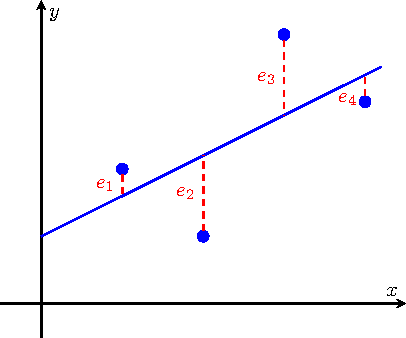
\includegraphics[width=\textwidth,page=1]{../Diagrams/least-square-regression-line/regression-line.pdf}
      \caption{\ref{Me} \ref{source:conics2} Regression line of \(y\) on \(x\).}
      \label{fig:y-on-x}
    \end{figure}
    The regression line of \(y\) on \(x\) assumes that the values of \(x\) are known exactly and to perfect accuracy. As such, it minimises the sum of squared \textcolor{red}{distances}, \(\sum{\textcolor{red}{e_i}^2}\) in the \(y\)-direction, as shown above.
  \end{minipage}\hfill
  \begin{minipage}{0.475\textwidth}
    \begin{figure}[H]
      \centering
      \includegraphics[width=\textwidth,page=2]{../Diagrams/least-square-regression-line/regression-line.pdf}
      \caption{\ref{Me} \ref{source:conics2} Regression line of \(x\) on \(y\).}
      \label{fig:x-on-y}
    \end{figure}
    The regression line of \(x\) on \(y\) assumes that the values of \(y\) are known exactly and to perfect accuracy. As such, it minimises the sum of squared \textcolor{red}{distances}, \(\sum{\textcolor{red}{e_i}^2}\) in the \(x\)-direction, as shown above.
  \end{minipage}
\end{note}
\begin{example}{}{}
  Show on the scatter diagram in part (d) the distances which are used in drawing the least squares regression line of \(y\) on \(x\). Explain why these distances are squared, and why this is referred to as the `method of least squares'.

  \rule{20cm-137.0549pt}{0.05mm}
  \begin{figure}[H]
      \centering
      \includegraphics[width=0.475\textwidth,page=3]{../Diagrams/least-square-regression-line/regression-line.pdf}
      \caption{\ref{Me} \ref{source:conics2} Regression line of \(y\) on \(x\).}
      \label{fig:least-squares}
  \end{figure}
  \begin{itemize}
    \item The \textcolor{red}{distances} are signed, i.e. can be positive or negative. 
    \item So, squaring the \textcolor{red}{distances} ensures the sum will not become zero (unless the plotted points are collinear) or negative.
    \item The least squares regression line is the line for which the sum of squared \textcolor{red}{distances} is minimised. Hence, this is referred to as the `method of least squares'
  \end{itemize} 
\end{example}
\begin{example}{}{}
  % N2003/II/11
  Suppose that we are given pairs of data for \(x\) and \(y\), as shown below:
  \begin{table}[H]
    \centering
    \begin{tabular}{ScScScScSc}
      \toprule
      \(x\) & \(x_1\) & \(x_2\) & \(\cdots\) & \(x_n\)\\
      \midrule
      \(y\) & \(y_1\) & \(y_2\) & \(\cdots\) & \(y_n\)\\
      \bottomrule
    \end{tabular}
    \caption{A dataset of \(n\) pairs of \(x\) and \(y\) values.}
  \end{table} 
  Let \(Y\) be the value obtained by substituting a sample value of \(x\) into the equation of the regression line of \(y\) on \(x\), given by \(Y=ax+b\). Consider any \(Y'=\alpha x+\beta\). What can you say about the value of \(\sum{(y-Y')^2}\)?

  \rule{\textwidth}{0.05mm}\vspace{0.5\baselineskip}
  Since \(\sum{(y-Y')^2}\) is minimised when \(Y'=ax+b\), we see that \(\sum{(y-Y')^2}\geq\sum{(y-Y)^2}\) for any \(Y'=\alpha x+\beta\).
\end{example}
\begin{note}
  The regression lines of \(y\) on \(x\) and \(x\) on \(y\) intersect at \((\widebar{x},\widebar{y})\).
\end{note}
\begin{note}
  To estimate the value of a variable \(y\), given a the value of another variable \(x\), we always use the regression line of the \hl[green!25]{\emph{dependent} variable} on the \hl[blue!15]{\emph{independent} variable}.
  \begin{table}[H]
    \centering
    \begin{tabular}{>{\columncolor{blue!15}}Sc>{\columncolor{green!25}}ScSc}
      \toprule
      Independent variable & Dependent variable & Regression line\\
      \midrule
      \(x\) & \(y\) & \(\highlight[green!25]{y}\) on \(\highlight[blue!15]{x}\)\\
      \(y\) & \(x\) & \(\highlight[green!25]{x}\) on \(\highlight[blue!15]{y}\)\\
      \bottomrule
    \end{tabular}
    \caption{Regression line to use for estimations.}
    \label{table:regression-line-indepedent-dependent-variable}
  \end{table}
\end{note}
\begin{note}
  Explain why a linear model would not be appropriate. Choose any relevant ones.
    \begin{itemize}
      \item The scatter diagram/data indicates that, as \(x\) increases, \(y\) [e.g. increases at a decreasing rate], which is \emph{not} a linear relationship.
      \item A linear model will increase \emph{indefinitely} with more [\(x\) in context]. This is contextually \emph{unrealistic}, as [reason in context]. 
      \item A linear model would imply that, in the long run, the [e.g. time taken] would be negative, which is impossible.
    \end{itemize}
\end{note}
\begin{note}
  By calculating the product moment correlation coefficients, explain whether model \(y=ax+b\) or model \(\mathbf{y}=\mathbf{a}\mathbf{x}+\mathbf{b}\) is more appropriate.
  \begin{center}
    \parbox{0.9\textwidth}{
      The \(\lvert r \rvert\) value for the model \(y=ax+b\) is higher at \rule{0.5cm}{0.01mm}, compared to \rule{0.5cm}{0.01mm} for the model \(\mathbf{y}=\mathbf{a}\mathbf{x}+\mathbf{b}\). Thus, there is a stronger (positive/negative) correlation between \(x\) and \(y\). As such, the model \(y=ax+b\) is more appropriate.
    }
  \end{center}
\end{note}
\begin{note}
  Let \(x\) be in unit\(_x\) and \(\mathbf{x}\) be in unit\(_{\mathbf{x}}\). Suppose that the \(c\text{ unit}_x=1\text{ unit}_\mathbf{x}\), where \(c\) is a constant. Then, if \(y=ax+b\), we have \(y=ac\mathbf{x}+b\).
\end{note}
\section{Other Notes}
\begin{note}
  Explain whether it is valid to conclude that a higher value of \(x\) will \emph{result in} a lower/higher value of \(y\).
  
  \begin{center}
    \parbox{0.9\textwidth}{
      No. While a higher value of \(x\) is \emph{correlated} with a higher value of \(y\), this does not imply any \emph{causal} relationship between \(x\) and \(y\).
    }
  \end{center}
  \emph{Note.} ``result in'' tends to refer to a \emph{causal} relationship.
\end{note}
\begin{example}{}{}
  Suggest an improvement to the data collection process so that the results could provide a fairer gauge of the expected outcome.
  \begin{center}
    \parbox{0.9\textwidth}{
      The randomly selected [members of population] might have been of different [category 1; e.g. gender] and [category 2; e.g. age]. To make the results fairer, the data could have been separated based on [category 1] and [category 2].
    }
  \end{center}
\end{example}